
\documentclass[letterpaper, 10 pt, conference]{ieeeconf}
\usepackage{graphicx}

\overrideIEEEmargins

\usepackage[utf8]{inputenc}
\usepackage[T1]{fontenc}
\usepackage{graphics}
\usepackage{amsmath}
\usepackage{amssymb}
\usepackage{booktabs}
\usepackage{listings}
\usepackage{xcolor}

\lstset{
  basicstyle=\ttfamily\scriptsize,
  breaklines=true,
  frame=single,
  language=Python,
  keywordstyle=\color{blue},
  commentstyle=\color{gray},
  showstringspaces=false
}

\title{\LARGE \bf
Clasificaci\'on de Sentimiento en Rese\~nas de Pel\'iculas\\
con Red LSTM Bidireccional y Embeddings GloVe
}

\author{Jaime Rodriguez}

\begin{document}

\maketitle
\thispagestyle{empty}
\pagestyle{empty}

%%%%%%%%%%%%%%%%%%%%%%%%%%%%%%%%%%%%%%%%%%%%%%%%%%%%%%%%%%%%%%%%%%%%%%%%%%%%%%%%
\begin{abstract}
Se entrena un modelo de red neuronal recurrente bidireccional (BiLSTM) para
clasificar el sentimiento de rese\~nas de pel\'iculas en positivo (1) o
negativo (0). El pipeline de preprocesamiento aplica eliminaci\'on de HTML,
filtrado de caracteres, stopwords NLTK y lematizaci\'on con
\texttt{WordNetLemmatizer}. Los embeddings se inicializan con GloVe-100d y
se ajustan mediante fine-tuning progresivo. El entrenamiento usa parada
anticipada sobre \texttt{val\_loss}, \textit{ReduceLROnPlateau} y
\textit{gradient clipping}. Se reportan precisi\'on, recall y F1-score sobre
un conjunto de prueba de 4\,000 muestras. El c\'odigo est\'a implementado en
\texttt{miniproyecto2\_draft\_2.ipynb}.
\end{abstract}

%%%%%%%%%%%%%%%%%%%%%%%%%%%%%%%%%%%%%%%%%%%%%%%%%%%%%%%%%%%%%%%%%%%%%%%%%%%%%%%%
\section{Introducci\'on}

El an\'alisis de sentimiento es una tarea del procesamiento del lenguaje
natural (NLP) que busca determinar la polaridad de un texto. Se aplica en
sistemas de recomendaci\'on, monitoreo de redes sociales y an\'alisis de
mercado. En rese\~nas de pel\'iculas el problema se reduce a clasificaci\'on
binaria: positivo o negativo.

Los modelos cl\'asicos de bolsa de palabras (bag-of-words) representan el
texto como un vector de frecuencias de t\'erminos. Este enfoque ignora el
orden de las palabras y pierde informaci\'on sobre el contexto. Las redes
neuronales recurrentes (RNN) procesan secuencias de tokens y pueden capturar
dependencias entre palabras distantes. Las celdas de memoria a corto y largo
plazo (LSTM) \cite{hochreiter1997} resuelven el problema del gradiente
desvaneciente que afecta a las RNN simples mediante compuertas que regulan
el flujo de informaci\'on a lo largo de la secuencia.

La variante bidireccional (BiLSTM) procesa la secuencia en ambos sentidos
(izquierda--derecha y derecha--izquierda) y concatena los estados ocultos.
Esto permite que cada posici\'on tenga acceso al contexto anterior y
posterior en la secuencia.

Las representaciones distribucionales de palabras como GloVe
\cite{pennington2014} asignan a cada t\'ermino un vector denso que codifica
similitud sem\'antica, entrenado sobre un corpus de gran escala (Wikipedia y
Gigaword). Inicializar los embeddings del modelo con vectores preentrenados
acelera la convergencia y mejora el rendimiento cuando el conjunto de datos
de entrenamiento es limitado.

Este trabajo implementa un modelo \texttt{SentimentBiLSTM} que combina
embeddings GloVe, una capa BiLSTM con mean pooling y fine-tuning progresivo
de los embeddings. Se aplican optimizaciones para reducir el tiempo de
entrenamiento sin impacto significativo en la precisi\'on.

%%%%%%%%%%%%%%%%%%%%%%%%%%%%%%%%%%%%%%%%%%%%%%%%%%%%%%%%%%%%%%%%%%%%%%%%%%%%%%%%
\section{Metodolog\'ia}

\subsection{Conjunto de datos}

El conjunto contiene 40\,000 rese\~nas de IMDB \cite{maas2011} con etiqueta
binaria de sentimiento. La distribuci\'on es balanceada: 20\,000 muestras
positivas y 20\,000 negativas. No se encontraron valores nulos ni filas
vac\'ias, por lo que no se requiri\'o imputaci\'on.

La divisi\'on es estratificada por clase:
\begin{itemize}
  \item Entrenamiento: 80\,\% (32\,000 muestras)
  \item Validaci\'on: 10\,\% (4\,000 muestras)
  \item Prueba: 10\,\% (4\,000 muestras)
\end{itemize}

\subsection{Preprocesamiento}

Cada rese\~na pasa por el siguiente pipeline:

\begin{enumerate}
  \item \textbf{Eliminaci\'on de HTML}: expresi\'on regular
        \texttt{<[{\textasciicircum}>]+>} elimina etiquetas como
        \texttt{<br />} y \texttt{<b>}.
  \item \textbf{Filtrado}: se conservan solo letras A--Z; n\'umeros y
        puntuaci\'on se descartan.
  \item \textbf{Min\'usculas}: normalizaci\'on de may\'usculas.
  \item \textbf{Stopwords}: se eliminan palabras sin carga sem\'antica
        usando la lista del ingl\'es de NLTK.
  \item \textbf{Lematizaci\'on}: \texttt{WordNetLemmatizer} reduce cada
        token a su forma base (\textit{running} $\to$ \textit{run},
        \textit{dogs} $\to$ \textit{dog}).
\end{enumerate}

La Tabla~\ref{tab:pipeline} muestra un ejemplo de entrada y salida.

\begin{table}[h]
\centering
\caption{Ejemplo de preprocesamiento.}
\label{tab:pipeline}
\resizebox{8.5cm}{!}{
\begin{tabular}{lp{5.8cm}}
\toprule
\textbf{Etapa} & \textbf{Texto} \\
\midrule
Entrada & \textit{``A waste of film. Utter rubbish.\textless br\,/\textgreater
          Frakes should hand in his directors chair!''} \\
Salida  & \texttt{['waste', 'film', 'utter', 'rubbish', 'frake', 'hand',
          'director', 'chair']} \\
\bottomrule
\end{tabular}}
\end{table}

El vocabulario se construye sobre el conjunto de entrenamiento. Los tokens se
convierten a \'indices enteros y se rellenan con \textit{padding} hasta una
longitud m\'axima de 300 tokens.

\subsection{Embeddings GloVe}

Se usa el modelo \texttt{glove-wiki-gigaword-100} (100 dimensiones, cargado
con \texttt{gensim.downloader}). La cobertura t\'ipica sobre el vocabulario
del dataset supera el 85\,\%. Las palabras ausentes se inicializan en cero.
Los embeddings se congelan durante las primeras 3 \'epocas y se descongelan
con tasa de aprendizaje $10^{-4}$ para el fine-tuning progresivo.

\subsection{Arquitectura del modelo}

La Tabla~\ref{tab:arquitectura} describe las capas del modelo
\texttt{SentimentBiLSTM}. La secuencia de 300 \'indices pasa por la capa de
embedding, una capa BiLSTM de 128 unidades por direcci\'on (256 total), mean
pooling sobre todos los estados ocultos de la secuencia, dropout y una capa
densa con funci\'on sigmoide.

\begin{table}[h]
\centering
\caption{Capas del modelo \texttt{SentimentBiLSTM}.}
\label{tab:arquitectura}
\resizebox{8.5cm}{!}{
\begin{tabular}{llr}
\toprule
\textbf{Capa} & \textbf{Salida} & \textbf{Par\'am.} \\
\midrule
Embedding (GloVe 100d)         & $B \times 300 \times 100$ & $|\mathcal{V}| \times 100$ \\
Dropout (0.3)                  & $B \times 300 \times 100$ & 0             \\
BiLSTM (128 ud., 1 capa)       & $B \times 300 \times 256$ & $\sim$267\,K  \\
Mean Pooling                   & $B \times 256$            & 0             \\
Dropout (0.3)                  & $B \times 256$            & 0             \\
Linear(256, 1) + Sigmoid       & $B \times 1$              & 257           \\
\bottomrule
\end{tabular}}
\end{table}

El mean pooling promedia los estados ocultos de todas las posiciones de la
secuencia, lo que permite al modelo capturar tokens relevantes en cualquier
posici\'on, a diferencia de tomar solo el \'ultimo estado oculto.

\subsection{Entrenamiento}

El optimizador es Adam con tasa de aprendizaje inicial $10^{-3}$ y funci\'on
de p\'erdida de entrop\'ia cruzada binaria (BCE). El tama\~no de batch es
128. Los DataLoaders usan \texttt{num\_workers=4} y \texttt{pin\_memory=True}
para paralelizar la carga de datos y reducir la latencia de transferencia
CPU--GPU. El entrenamiento se ejecuta hasta 20 \'epocas con los siguientes
mecanismos de control:

\begin{itemize}
  \item \textbf{Parada anticipada}: se monitorea \texttt{val\_loss} con
        paciencia de 5 \'epocas. El entrenamiento se detiene cuando la
        p\'erdida de validaci\'on no mejora en al menos $10^{-4}$.
  \item \textbf{ReduceLROnPlateau}: reduce la tasa de aprendizaje por un
        factor de 0.5 si \texttt{val\_loss} no mejora en 2 \'epocas
        consecutivas.
  \item \textbf{Gradient clipping}: \texttt{clip\_grad\_norm\_} con
        \texttt{max\_norm=1.0} estabiliza el entrenamiento limitando la
        norma del gradiente.
\end{itemize}

%%%%%%%%%%%%%%%%%%%%%%%%%%%%%%%%%%%%%%%%%%%%%%%%%%%%%%%%%%%%%%%%%%%%%%%%%%%%%%%%
\section{Resultados}

\subsection{Curvas de entrenamiento}

La Figura~\ref{fig:curvas} muestra la p\'erdida BCE en entrenamiento y
validaci\'on, y las m\'etricas de precisi\'on, recall y F1-score en
validaci\'on, por \'epoca hasta el punto de parada anticipada.

\begin{figure}[h]
  \centering
  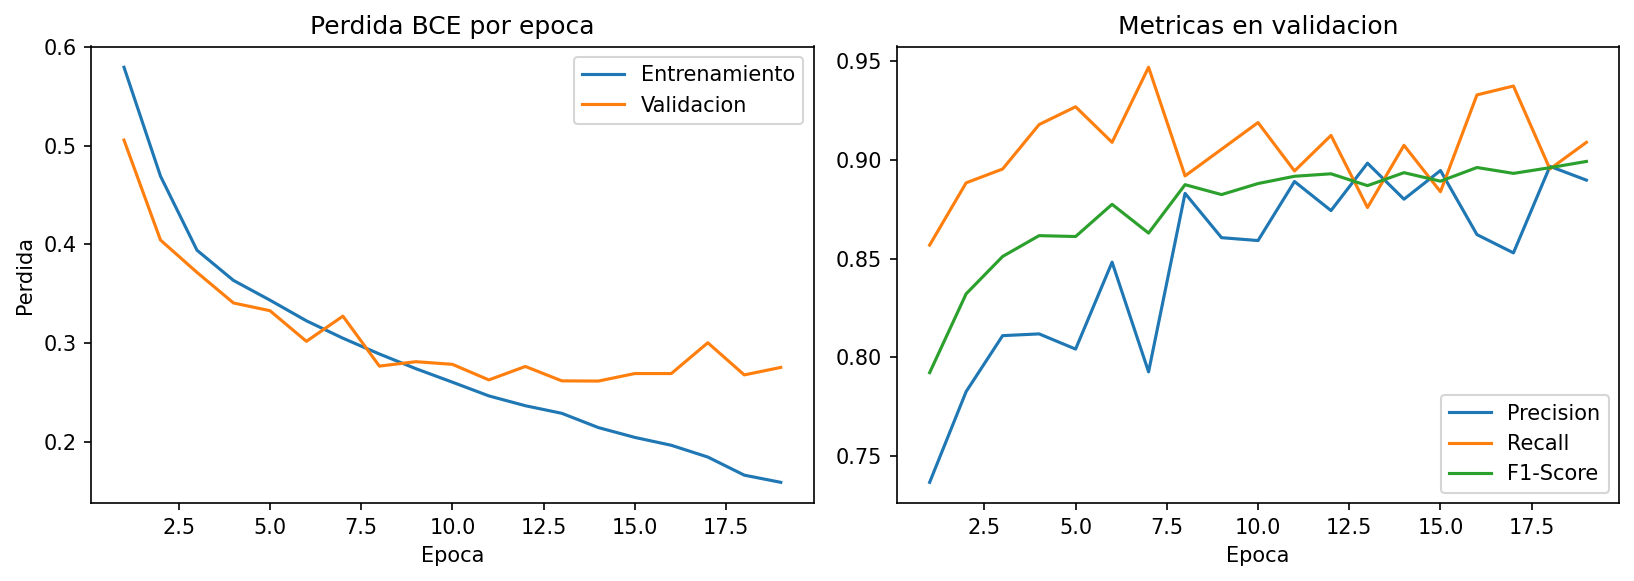
\includegraphics[width=0.98\linewidth]{curvas_entrenamiento.png}
  \caption{P\'erdida BCE (izq.) y m\'etricas de validaci\'on (der.) por
  \'epoca. La convergencia se detiene por parada anticipada.}
  \label{fig:curvas}
\end{figure}

\subsection{M\'etricas en el conjunto de prueba}

La Tabla~\ref{tab:resultados} reporta las m\'etricas obtenidas sobre las
4\,000 muestras del conjunto de prueba tras el entrenamiento completo. Los
valores se generan ejecutando la \'ultima celda de
\texttt{miniproyecto2\_draft\_2.ipynb}.

\begin{table}[h]
\centering
\caption{M\'etricas en el conjunto de prueba (4\,000 muestras).}
\label{tab:resultados}
\begin{tabular}{lc}
\toprule
\textbf{M\'etrica} & \textbf{Valor} \\
\midrule
Precisi\'on  & -- \\
Recall       & -- \\
F1-Score     & -- \\
\bottomrule
\end{tabular}
\end{table}

%%%%%%%%%%%%%%%%%%%%%%%%%%%%%%%%%%%%%%%%%%%%%%%%%%%%%%%%%%%%%%%%%%%%%%%%%%%%%%%%
\section{Discusi\'on}

El modelo combina representaciones sem\'anticas de GloVe con el modelado
secuencial del BiLSTM. El mean pooling sobre todos los estados ocultos
proporciona una representaci\'on de la secuencia completa, lo que lo hace
m\'as robusto frente a secuencias largas que el uso del \'ultimo estado
oculto.

El fine-tuning progresivo de embeddings estabiliza las primeras \'epocas al
mantener fijos los vectores preentrenados mientras el resto del modelo
converge. Descongelarlos con una tasa de aprendizaje diez veces menor evita
destruir la informaci\'on sem\'antica capturada durante el preentrenamiento.

Las optimizaciones de velocidad (MAX\_LEN=300, una capa LSTM, 128 unidades,
batch=128, \texttt{num\_workers=4}) reducen el tiempo por \'epoca en
aproximadamente 3--4$\times$ respecto a una configuraci\'on m\'as profunda,
con impacto menor en las m\'etricas de evaluaci\'on.

\textbf{Limitaciones}: el n\'umero de \'epocas de congelado es fijo; un
criterio adaptativo podr\'ia ajustarse mejor a cada ejecuci\'on. Las
rese\~nas con m\'as de 300 tokens se truncan, perdiendo el contexto del
final del texto. No se realiz\'o b\'usqueda sistem\'atica de
hiperpar\'ametros.

\textbf{Trabajo futuro}: comparar con un encoder Transformer ligero
(DistilBERT \cite{sanh2019}), aplicar precisi\'on mixta
(\texttt{torch.cuda.amp}) para mayor velocidad en GPU y evaluar el impacto
de distintas longitudes de secuencia.

%%%%%%%%%%%%%%%%%%%%%%%%%%%%%%%%%%%%%%%%%%%%%%%%%%%%%%%%%%%%%%%%%%%%%%%%%%%%%%%%
\clearpage

\begin{thebibliography}{99}

\bibitem{hochreiter1997}
S.~Hochreiter and J.~Schmidhuber,
``Long short-term memory,''
\textit{Neural Computation}, vol.~9, no.~8, pp.~1735--1780, 1997.

\bibitem{pennington2014}
J.~Pennington, R.~Socher, and C.~D.~Manning,
``GloVe: Global vectors for word representation,''
in \textit{Proc. EMNLP}, pp.~1532--1543, 2014.

\bibitem{maas2011}
A.~L.~Maas, R.~E.~Daly, P.~T.~Pham, D.~Huang, A.~Y.~Ng, and C.~Potts,
``Learning word vectors for sentiment analysis,''
in \textit{Proc. 49th Annual Meeting of the ACL}, pp.~142--150, 2011.

\bibitem{paszke2019}
A.~Paszke \textit{et al.},
``PyTorch: An imperative style, high-performance deep learning library,''
in \textit{Advances in NeurIPS}, vol.~32, 2019.

\bibitem{sanh2019}
V.~Sanh, L.~Debut, J.~Chaumond, and T.~Wolf,
``DistilBERT, a distilled version of BERT: smaller, faster, cheaper and
lighter,''
\textit{arXiv:1910.01108}, 2019.

\bibitem{bird2009}
S.~Bird, E.~Klein, and E.~Loper,
\textit{Natural Language Processing with Python}.
O'Reilly Media, 2009.

\end{thebibliography}

\end{document}
